\documentclass[tikz,border=10pt]{standalone}
\usepackage{sourcesanspro}
\usepackage[T1]{fontenc}
\usetikzlibrary{arrows.meta, positioning}

\definecolor{inkslate}{HTML}{1C212B}
\definecolor{steel}{HTML}{45505F}
\definecolor{bootcol}{HTML}{AD5A2B}
\definecolor{bootcolsoft}{HTML}{F4E3D3}
\definecolor{pmucol}{HTML}{1F6F6B}
\definecolor{pmucolsoft}{HTML}{D7E8E6}

\begin{document}
\sffamily
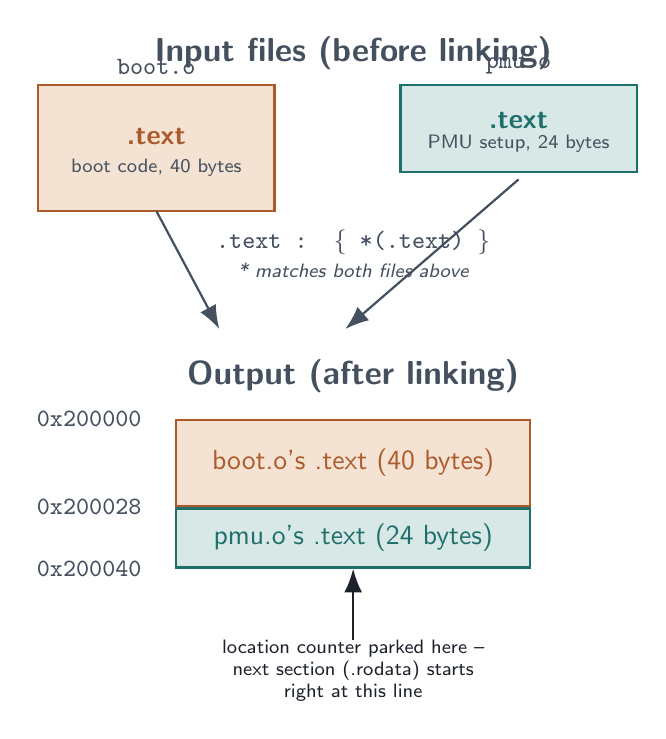
\begin{tikzpicture}[font=\sffamily\small]

  % ---------- Title ----------
  \node[font=\sffamily\bfseries\large\color{steel}] at (4.3,5.0) {Input files (before linking)};

  % ---------- boot.o block ----------
  \node[draw=bootcol, fill=bootcolsoft, thick, minimum width=3cm, minimum height=1.6cm,
        label={[color=steel]above:\texttt{boot.o}}] (bootbox) at (1.8,3.8) {};
  \node[color=bootcol, font=\sffamily\bfseries] at (1.8,3.95) {.text};
  \node[color=steel, font=\sffamily\scriptsize] at (1.8,3.55) {boot code, 40 bytes};

  % ---------- pmu.o block ----------
  \node[draw=pmucol, fill=pmucolsoft, thick, minimum width=3cm, minimum height=1.1cm,
        label={[color=steel]above:\texttt{pmu.o}}] (pmubox) at (6.4,4.05) {};
  \node[color=pmucol, font=\sffamily\bfseries] at (6.4,4.15) {.text};
  \node[color=steel, font=\sffamily\scriptsize] at (6.4,3.85) {PMU setup, 24 bytes};

  % ---------- linker script line ----------
  \node[color=steel, font=\sffamily\ttfamily\small] at (4.3,2.6)
    {.text : \{ *(.text) \}};
  \node[color=steel, font=\sffamily\scriptsize\itshape] at (4.3,2.25)
    {* matches both files above};

  \draw[-{Latex[length=3mm]}, thick, color=steel] (1.8,3.0) -- (2.6,1.5);
  \draw[-{Latex[length=3mm]}, thick, color=steel] (6.4,3.4) -- (4.2,1.5);

  % ---------- Title 2 ----------
  \node[font=\sffamily\bfseries\large\color{steel}] at (4.3,0.9) {Output (after linking)};

  % ---------- output stack ----------
  \node[draw=bootcol, fill=bootcolsoft, thick, minimum width=4.5cm, minimum height=1.1cm] (outboot) at (4.3,-0.2) {};
  \node[color=bootcol, font=\sffamily] at (4.3,-0.2) {boot.o's .text (40 bytes)};

  \node[draw=pmucol, fill=pmucolsoft, thick, minimum width=4.5cm, minimum height=0.75cm, below=0pt of outboot] (outpmu) {};
  \node[color=pmucol, font=\sffamily] at (outpmu) {pmu.o's .text (24 bytes)};

  % ---------- address labels ----------
  \node[anchor=east, font=\ttfamily\small, color=steel] at ([xshift=-0.3cm]outboot.north west) {0x200000};
  \node[anchor=east, font=\ttfamily\small, color=steel] at ([xshift=-0.3cm]outpmu.north west) {0x200028};
  \node[anchor=east, font=\ttfamily\small, color=steel] at ([xshift=-0.3cm]outpmu.south west) {0x200040};

  % ---------- location counter arrow ----------
  \draw[-{Latex[length=3mm]}, thick, color=inkslate] ([yshift=-0.9cm]outpmu.south) -- (outpmu.south);
  \node[color=inkslate, font=\sffamily\scriptsize, align=center] at ([yshift=-1.3cm]outpmu.south)
    {location counter parked here --\\next section (.rodata) starts\\right at this line};

\end{tikzpicture}
\end{document}
